%!TEX program = pdflatex
%# -*- coding: utf-8 -*-
%!TEX encoding = UTF-8 Unicode

\documentclass[12pt,oneside,a4paper]{article}

%% ------------------------------------------------------
%% load packages
\usepackage{geometry}
\geometry{verbose,tmargin=2cm,bmargin=2cm,lmargin=2cm,rmargin=2cm}
\usepackage[pdfusetitle,
 bookmarks=true,bookmarksnumbered=true,bookmarksopen=true,bookmarksopenlevel=2,
 breaklinks=false,pdfborder={0 0 1},backref=false,colorlinks=false,
 unicode=true]
 {hyperref}
\hypersetup{pdfstartview={XYZ null null 1}}
\usepackage{url}
\setcounter{secnumdepth}{2}
\setcounter{tocdepth}{2}
\usepackage{microtype}

\usepackage{amsmath, amsthm, amssymb, amsfonts}
\usepackage[retainorgcmds]{IEEEtrantools}
\usepackage{bbm}

% \usepackage{algorithm}
% \usepackage{algorithmic}
% \renewcommand{\algorithmicrequire}{\textbf{Input:}}
% \renewcommand{\algorithmicensure}{\textbf{Output:}}
\usepackage[algoruled, vlined]{algorithm2e}

\usepackage[T1]{fontenc}
\usepackage[utf8]{inputenc}
\usepackage[mono=false]{libertine}
\usepackage[libertine]{newtxmath}
\linespread{1.05}
\setlength{\parskip}{.5\baselineskip}
% \usepackage[toc,eqno,enum,bib,lineno]{tabfigures}

\usepackage{graphics}
\usepackage{graphicx}
\usepackage[figure]{hypcap}
\usepackage[hypcap]{caption}
\usepackage{tikz}
\usepackage{tikz-cd}
%\usepackage{grffile}
%\usepackage{float}
\usepackage{pdfpages}
\usepackage{pdflscape}
\usepackage{needspace}

\usepackage{multirow}
\usepackage{booktabs}
\usepackage{threeparttable}
\usepackage{dcolumn}
\usepackage{tabu}

\usepackage{verbatim}

% \usepackage[square,numbers,super,comma,sort]{natbib}
\usepackage[backend=biber, style=nature, sorting=none, isbn=false, url=false, doi=false]{biblatex}
\addbibresource{ref.bib}
\usepackage[]{authblk}

%% Class, Exam, Date, etc.
\newcommand{\class}{CSCI 5525: Machine Learning}
\newcommand{\term}{Fall 2015}
\newcommand{\examnum}{Homework 3}
\newcommand{\hmwkTitle}{\class \\[1ex] \examnum}
\newcommand{\hmwkAuthorName}{Jingxiang Li}

\title{\hmwkTitle}
\author{\hmwkAuthorName}

\usepackage{fancyhdr}
\usepackage{extramarks}
\lhead{\hmwkAuthorName}
\chead{}
\rhead{\hmwkTitle}
\cfoot{\thepage}

\newcounter{problemCounter}
\newcounter{subproblemCounter}
\renewcommand{\thesubproblemCounter}{\alph{subproblemCounter}}
\newcommand{\problem}[0] {
    \clearpage
    \stepcounter{problemCounter}
    \setcounter{subproblemCounter}{0}
}

\newcommand{\subproblem}[0] {
    \stepcounter{subproblemCounter}
    \noindent{\textbf{\large{Problem \theproblemCounter.\hspace{1pt}\thesubproblemCounter}}}
    \vspace{\baselineskip}
    \newline
}

\newcommand{\solution} {
    \vspace{15pt}
    \noindent\ignorespaces\textbf{\large Solution}\par
}
\setlength\parindent{0pt}

%% some math shortcuts
\newcommand{\m}[1]{\texttt{{#1}}}
\newcommand{\E}[0]{\mathrm{E}}
\newcommand{\Var}[0]{\mathrm{Var}}
\newcommand{\sd}[0]{\mathrm{sd}}
\newcommand{\Cov}[0]{\mathrm{Cov}}
%%%%%%%%%%%%%%%%%%%%%%%%%%%%%%%%%%%%%%%%%%%%%%%%%%%%%%%%%%%%%%%%%%%%%%%%%%%

\begin{document}
\maketitle

\problem
\subproblem
Knowing that for adaboost algorithm, we have
$$\frac{1}{N}\sum_{i = 1}^{N}{\mathbbm{1}(g(x_{i}) \neq y)} \leq \frac{1}{N}\sum_{i = 1}^{N}{\exp(-y_{i}g(x_{i}))} = \prod_{i = 1}^{T}Z_{t}$$
Where
$$Z_{t} = \sum_{i = 1}^{N}\exp(-\alpha_{t}y_{i}g_{t}(x_{i}))$$
is the normalization constant when update $w_{t + 1}(i)$

To minimize the training error, we minimize its upper-bound $\prod_{i = 1}^{T}Z_{t}$, i.e. find the best $\alpha_{t}$ that minimizing each $Z_{t}$, $t = 1,...,T$

Note that

\begin{equation*}
\begin{aligned}
Z_{t} & = \sum_{i = 1}^{N}\exp(-\alpha_{t}y_{i}g_{t}(x_{i})) = e^{-\alpha_{t}}\sum_{y_{i} = g_{t}(x_{i})}{w_{t}(i)} + e^{\alpha_{t}}\sum_{y_{i} \neq g_{t}(x_{i})}{w_{t}(i)}\\
& = (e^{\alpha_{t}} - e^{-\alpha_{t}}) \sum_{i = 1}^{N}{w_{t}(i)\mathbbm{1}(y_{i} \neq g_{t}(x_{i}))} + e^{-\alpha_{t}}\sum_{i = 1}^{N}{w_{t}(i)}\\
&= (e^{\alpha_{t}} - e^{-\alpha_{t}}) \epsilon_{t} + e^{-\alpha_{t}}
\end{aligned}
\end{equation*}

where
$$\epsilon_{t} = P_{x \sim w_{t}}(y \neq g_{t}(x)) =  \frac{\sum_{i = 1}^{N}{w_{t}(i)\mathbbm{1}(y_{i} \neq g_{t}(x_{i}))}}{\sum_{i = 1}^{N}{w_{t}(i)}}$$
Let $\beta = e^{\alpha_{t}}$, we try to solve the following optimization problem
$$\arg\min_{\beta}{f(\beta)} = (\beta - \frac{1}{\beta}) \epsilon_{t} + \frac{1}{\beta}$$
Let
$$\triangledown{f(\beta)} = \epsilon_{t} + (1 - \epsilon_{t})\frac{1}{\beta} = 0$$
We have
$$\beta = \sqrt{\frac{1 - \epsilon_{t}}{\epsilon_{t}}}$$
i.e.
$$\alpha_{t} = \log(\beta) = \frac{1}{2}\log(\frac{1 - \epsilon_{t}}{\epsilon_{t}})$$

Then we have
$$Z_{t} = (e^{\alpha_{t}} - e^{-\alpha_{t}}) \epsilon_{t} + e^{-\alpha_{t}} = 2\sqrt{\epsilon_{t}(1 - \epsilon_{t})}$$
Since $\epsilon_{t} \leq \frac{1}{2} - \frac{\gamma}{2}$
We have
$$Z_{t} \leq \sqrt{(1 - \gamma)(1 + \gamma)} = \sqrt{1 - \gamma^{2}}$$

Then we know
\begin{equation*}
\begin{aligned}
\frac{1}{N}\sum_{i = 1}^{N}{\mathbbm{1}(g(x_{i}) \neq y)} &\leq \prod_{i = 1}^{T}Z_{t} \leq \prod_{t = 1}^{T}{\sqrt{1 - \gamma^{2}}}\\
&= \exp(\log(\prod_{t = 1}^{T}{\sqrt{1 - \gamma^{2}}}))\\
&= \exp(\frac{1}{2}\sum_{t = 1}^{T}{\log(1 - \gamma^{2})})
\end{aligned}
\end{equation*}

Knowing that $\log(1 + x) \leq x$, $\forall x \in (-1, 0)$ and $-\gamma^{2} \in (-1, 0)$, we have
$$\frac{1}{N}\sum_{i = 1}^{N}{\mathbbm{1}(g(x_{i}) \neq y)} \leq \exp(-\frac{1}{2}\sum_{t = 1}^{T}{\gamma^{2}}) = \exp(-\frac{\gamma^{2}}{2}T)$$\\
Q.E.D.
\newline

\subproblem
Yes, since for adaboost algorithm we have proved that
$$\frac{1}{N}\sum_{i = 1}^{N}{\mathbbm{1}(g(x_{i}) \neq y)} \leq \exp(-\frac{\gamma^{2}}{2}T) \rightarrow 0, ~~T \rightarrow \infty$$
and the left hand side term is exactly the training error. Thus training error always become 0 as $T$ increases.\\
Q.E.D.
\newline


\problem
\subproblem
Before deriving the algorithm for Bagging and Random Forest, we need to define the information gain of a continuous random variable $X$

Let $H(Y)$ be the entropy of a random variable $Y$,
$$H(Y) = \sum_{i = 1}^{n}-p(y_{i})\log_{2}p(y_{i})$$
Then the conditional entropy $H(Y|X)$, which is the entropy of $Y$ given a discrete random variable $X$ is
$$H(Y|X) = \sum_{j = 1}^{m}p(x_{j})H(Y|x_{j})$$
If $X$ is a numeric random variable, we approximate $H(Y|X)$ by discretizing $X$ into a binary value random variable, i.e.
$$H(Y|X, C) = p(X < C)H(Y|X < C) + p(X \geq C)H(Y| X > C)$$
Then the information gain is defined as
$$IG(Y | X, C) = H(Y) - H(Y | X, C)$$
We will choose $C$ that maximize the information gain $IG(Y | X, C)$, i.e.
$$IG(Y | X) = \max_{C}IG(Y | X, C)$$
The optimization problem is solved by brute force search.

Then we will give a algorithm for training single binary split tree, which will be used for both Bagging and Random Forest.
\newline

\begin{algorithm}
\SetKwInOut{Input}{input}\SetKwInOut{Output}{output}
\Input{Design Matrix $X$ of size $n \times p$, Response Vector $y$ of size $n$, size of random feature set $M$, depth of the tree $D$}
\Output{Root of the Tree}
\If{$D \neq 0$}{
    Randomly pick $M$ features from $X$\\
    \ForEach{$j$ as the feature index}{
        $x = X[, j]$\\
        find the best split point $C_{j}$ and the corresponding information gain $Gain_{j}$ by minimizing $p(x < C_{j})H(y|x < C_{j}) + p(x \geq C_{j})H(y| x > C_{j})$\\
    }
    $J = \arg\max_{j}{Gain_{j}}$\\
    $X_l = X[X[, J] < C_{J}, :]$, $X_r = X[X[, J] \geq C_{J}, :]$\\
    Build Sub Trees with $X_l$, $X_r$ and depth $D - 1$
}
\caption{Binary Split Tree}\label{algo_tree}
\end{algorithm}
\clearpage

\emph{Bagging}
\begin{algorithm}
\SetKwInOut{Input}{input}\SetKwInOut{Output}{output}
\Input{Design Matrix $X$ of size $n \times p$, Response Vector $y$ of size $n$, number of base classifiers $B$,
size of random feature set $M = p$, depth of the tree $D$}
\Output{Bagging of the Trees}
\For{$i = 1, \dots B$}{
    Draw Bootstrap Sample From $X$ to form $X_{bootstrap}$ and $y_{bootstrap}$\\
    Build Binary Tree with $X_{bootstrap}$, $y_{bootstrap}$, $M = p$ and $D = D$\\
}
\caption{Bagging}\label{algo_bg}
\end{algorithm}

\emph{Simulation Result}

Here we run simulations for Bagging with different number of base classifiers, the result is summarized in figure \ref{fig:bg} and table \ref{tab:bg}. From the result we could see that the training and test error do not change significantly as the number of base classifiers increase, due to the fact the trees built in the Bagging algorithm are highly correlated.

\begin{figure}[ht!]
    \centering
    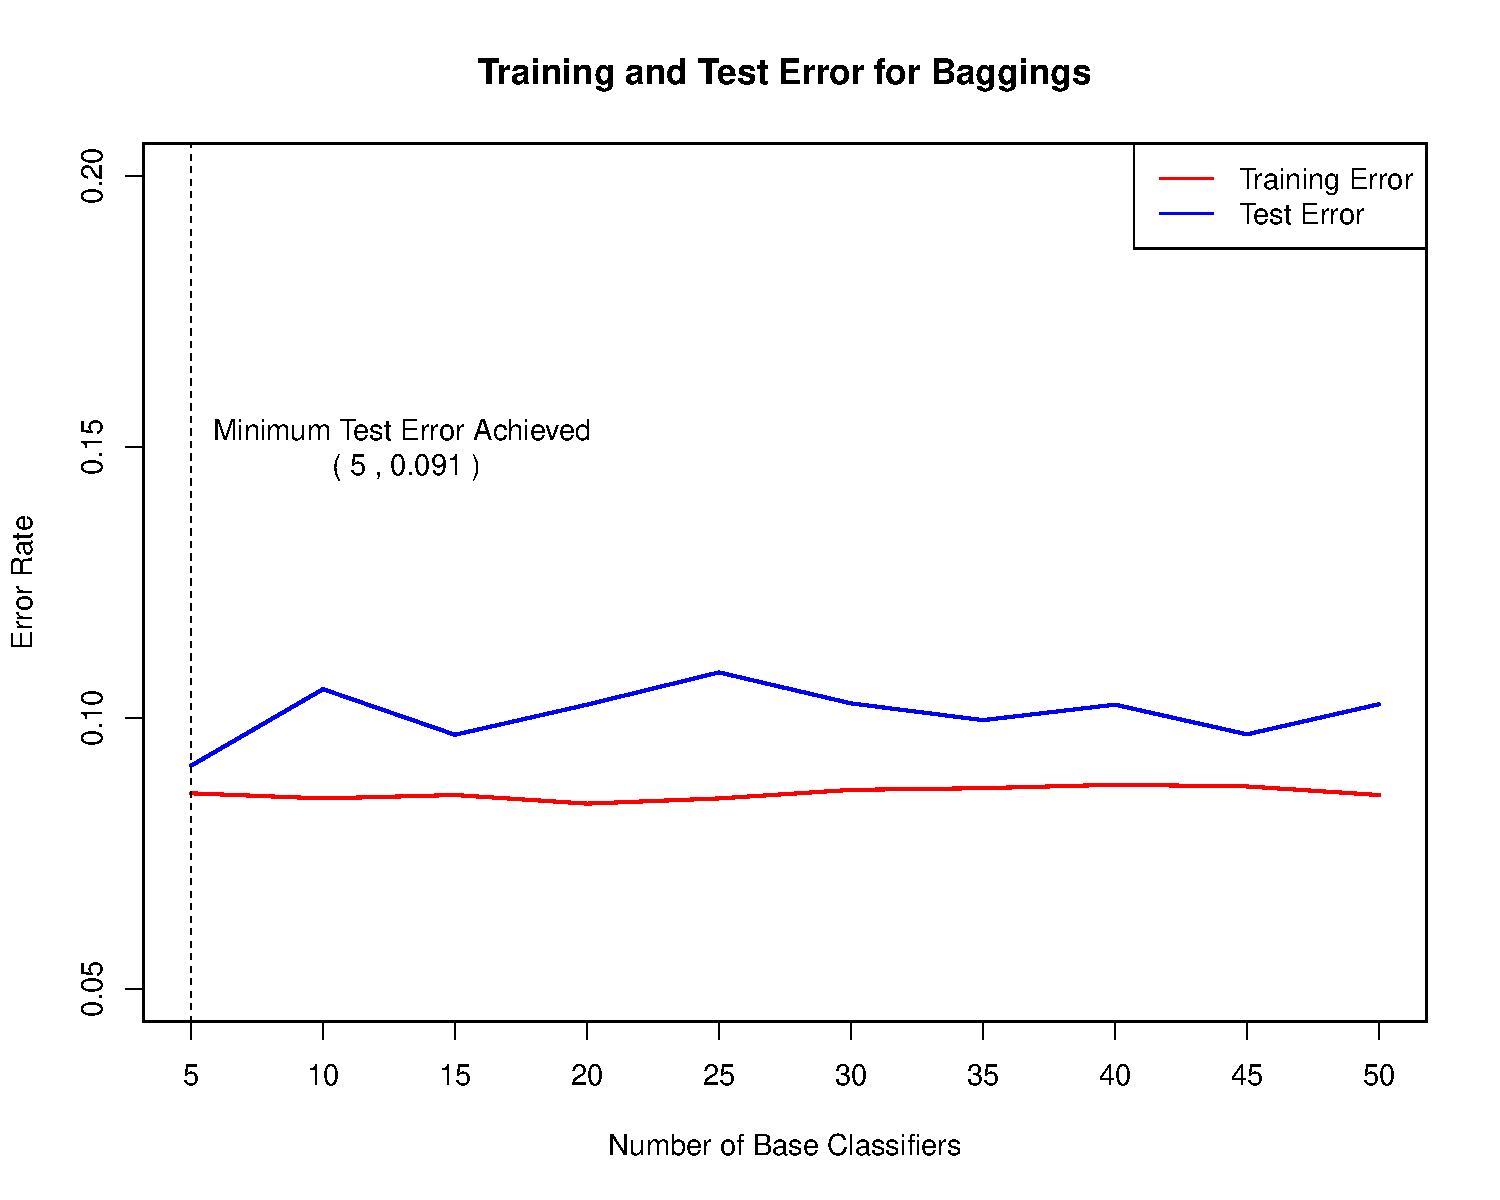
\includegraphics[width=1\textwidth]{./figure/bg.pdf}
    \caption{Simulation Result for Bagging}
    \label{fig:bg}
\end{figure}

\begin{table}[ht]
\centering
\caption{Simulation Result for Bagging}
\begin{tabular}{lrrrrrrrrrr}
  \toprule
 & \multicolumn{10}{c}{Number of Base Classifiers}\\
 \cmidrule[0.05em]{2-11}
Errors & 5 & 10 & 15 & 20 & 25 & 30 & 35 & 40 & 45 & 50 \\
  \midrule
Fold 1 Training & 0.092 & 0.092 & 0.086 & 0.076 & 0.095 & 0.086 & 0.083 & 0.079 & 0.095 & 0.089 \\
  Fold 1 Test & 0.083 & 0.139 & 0.083 & 0.139 & 0.056 & 0.056 & 0.139 & 0.139 & 0.056 & 0.111 \\
  Fold 2 Training & 0.089 & 0.098 & 0.092 & 0.092 & 0.085 & 0.085 & 0.092 & 0.085 & 0.089 & 0.092 \\
  Fold 2 Test & 0.086 & 0.057 & 0.143 & 0.086 & 0.143 & 0.143 & 0.086 & 0.143 & 0.086 & 0.057 \\
  Fold 3 Training & 0.085 & 0.092 & 0.085 & 0.076 & 0.092 & 0.089 & 0.082 & 0.089 & 0.089 & 0.082 \\
  Fold 3 Test & 0.114 & 0.171 & 0.086 & 0.057 & 0.086 & 0.114 & 0.143 & 0.114 & 0.086 & 0.143 \\
  Fold 4 Training & 0.089 & 0.098 & 0.092 & 0.079 & 0.060 & 0.085 & 0.085 & 0.085 & 0.089 & 0.089 \\
  Fold 4 Test & 0.114 & 0.029 & 0.114 & 0.114 & 0.086 & 0.143 & 0.029 & 0.200 & 0.114 & 0.143 \\
  Fold 5 Training & 0.079 & 0.095 & 0.089 & 0.076 & 0.076 & 0.085 & 0.089 & 0.092 & 0.082 & 0.098 \\
  Fold 5 Test & 0.171 & 0.086 & 0.086 & 0.200 & 0.229 & 0.057 & 0.086 & 0.086 & 0.114 & 0.029 \\
  Fold 6 Training & 0.098 & 0.070 & 0.054 & 0.082 & 0.095 & 0.085 & 0.092 & 0.095 & 0.092 & 0.082 \\
  Fold 6 Test & 0.057 & 0.114 & 0.086 & 0.171 & 0.029 & 0.143 & 0.057 & 0.029 & 0.086 & 0.171 \\
  Fold 7 Training & 0.085 & 0.085 & 0.101 & 0.092 & 0.089 & 0.082 & 0.085 & 0.085 & 0.082 & 0.085 \\
  Fold 7 Test & 0.114 & 0.114 & 0.029 & 0.057 & 0.086 & 0.143 & 0.143 & 0.114 & 0.171 & 0.143 \\
  Fold 8 Training & 0.089 & 0.047 & 0.092 & 0.092 & 0.085 & 0.098 & 0.092 & 0.092 & 0.089 & 0.089 \\
  Fold 8 Test & 0.000 & 0.086 & 0.114 & 0.029 & 0.171 & 0.029 & 0.114 & 0.086 & 0.086 & 0.086 \\
  Fold 9 Training & 0.066 & 0.095 & 0.085 & 0.079 & 0.092 & 0.089 & 0.082 & 0.085 & 0.079 & 0.095 \\
  Fold 9 Test & 0.057 & 0.086 & 0.057 & 0.143 & 0.086 & 0.057 & 0.114 & 0.086 & 0.114 & 0.057 \\
  Fold 10 Training & 0.089 & 0.079 & 0.082 & 0.098 & 0.082 & 0.082 & 0.089 & 0.089 & 0.089 & 0.057 \\
  Fold 10 Test & 0.114 & 0.171 & 0.171 & 0.029 & 0.114 & 0.143 & 0.086 & 0.029 & 0.057 & 0.086 \\
  Training Mean & 0.086 & 0.085 & 0.086 & 0.084 & 0.085 & 0.087 & 0.087 & 0.088 & 0.087 & 0.086 \\
  Training Std & 0.008 & 0.016 & 0.012 & 0.008 & 0.011 & 0.005 & 0.004 & 0.004 & 0.005 & 0.011 \\
  Test Mean & 0.091 & 0.105 & 0.097 & 0.102 & 0.108 & 0.103 & 0.100 & 0.102 & 0.097 & 0.103 \\
  Test Std & 0.046 & 0.046 & 0.041 & 0.060 & 0.059 & 0.047 & 0.038 & 0.052 & 0.034 & 0.047 \\
   \bottomrule
\end{tabular}
\label{tab:bg}
\end{table}
\clearpage

\emph{Random Forest}

\begin{algorithm}
\SetKwInOut{Input}{input}\SetKwInOut{Output}{output}
\Input{Design Matrix $X$ of size $n \times p$, Response Vector $y$ of size $n$, number of base classifiers $B$,
size of random feature set $M$, depth of the tree $D$}
\Output{Bagging of the Trees}
\For{$i = 1, \dots B$}{
    Draw Bootstrap Sample From $X$ to form $X_{bootstrap}$ and $y_{bootstrap}$\\
    Build Binary Tree with $X_{bootstrap}$, $y_{bootstrap}$, $M$ and $D$\\
}
\caption{Random Forest}\label{algo_rf}
\end{algorithm}

Here we run simulations for Random Forest with different size of random features, the result is summarized in figure \ref{fig:rf} and table \ref{tab:rf1}, \ref{tab:rf2}. From the result we could see that the training and test error first decrease, and then increase as the size of random features increases. Compared with Bagging, Random Forest has better generalization power in this case, since Random Forest is capable to de-correlate trees in the algorithm by randomly select features while training each node of the tree.


\begin{figure}[ht!]
    \centering
    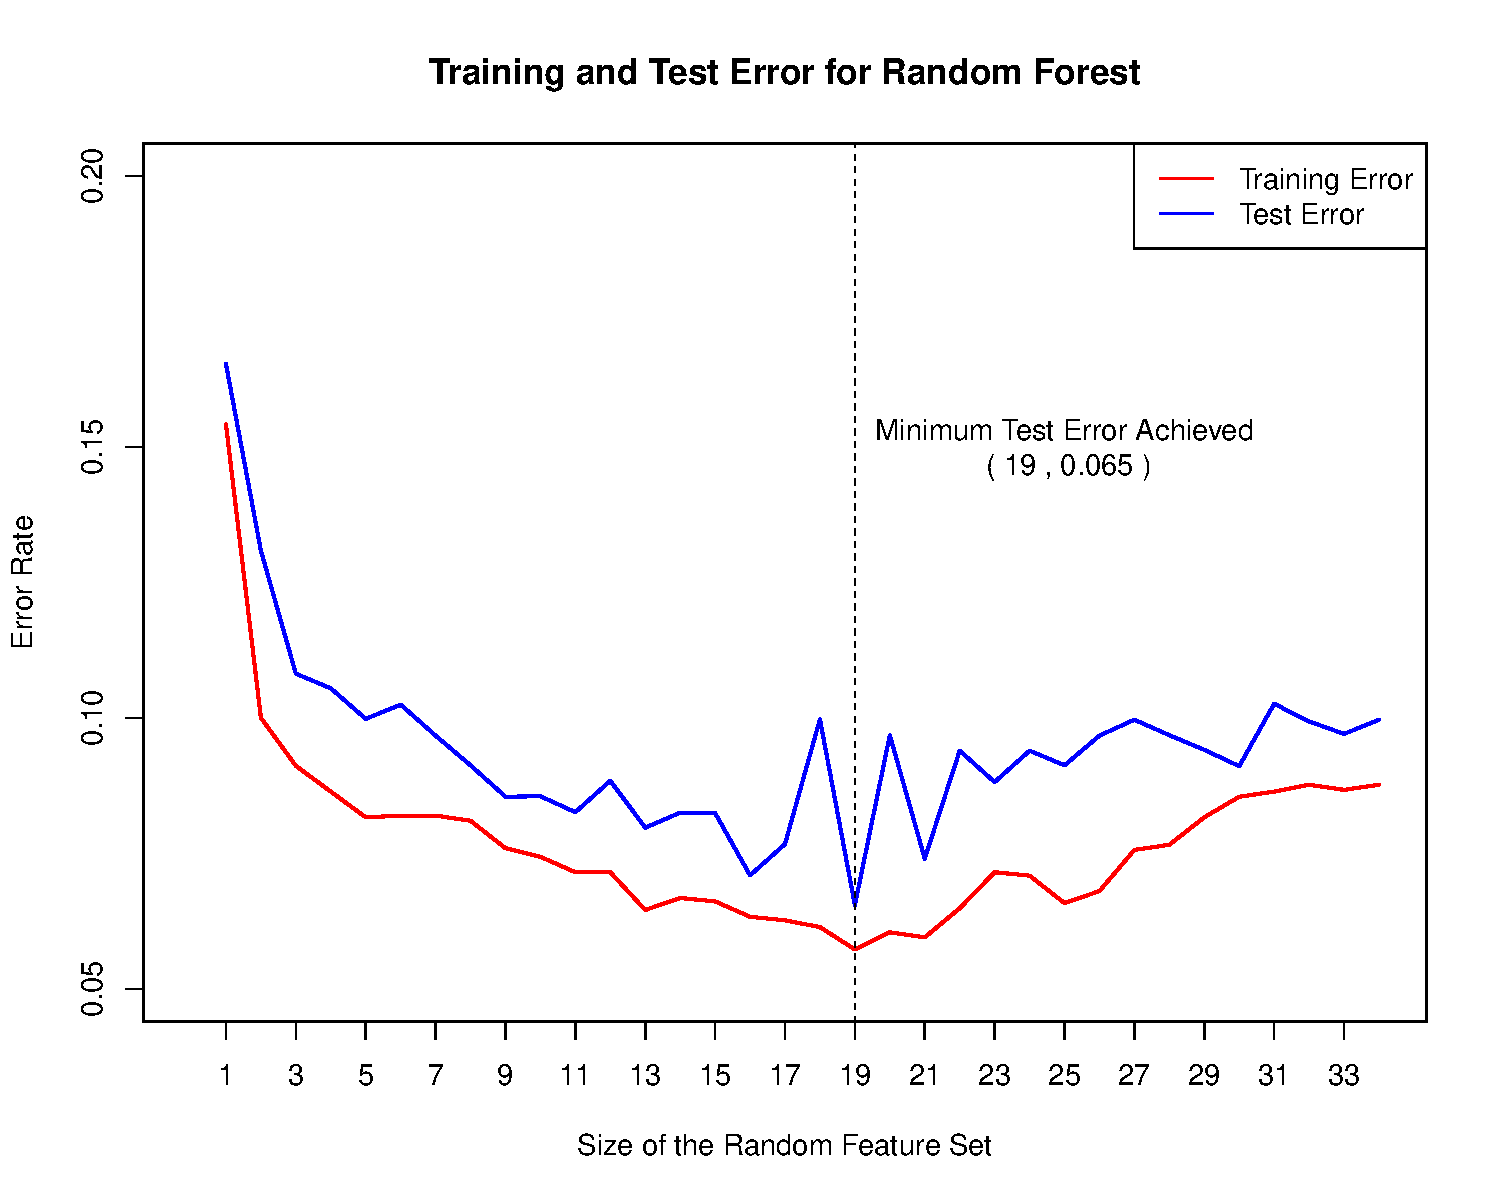
\includegraphics[width=1\textwidth]{./figure/rf.pdf}
    \caption{Simulation Result for Random Forest}
    \label{fig:rf}
\end{figure}

\begin{landscape}
\begin{table}[ht]
\centering
\caption{Simulation Result for Random Forest, Part 1}
\begin{tabular}{lrrrrrrrrrrrrrrrrr}
  \toprule
 & \multicolumn{17}{c}{Size of the Random Feature Set}\\
 \cmidrule[0.05em]{2-18}
Errors & 1 & 2 & 3 & 4 & 5 & 6 & 7 & 8 & 9 & 10 & 11 & 12 & 13 & 14 & 15 & 16 & 17 \\
  \midrule
Fold 1 Training & 0.165 & 0.098 & 0.108 & 0.086 & 0.079 & 0.076 & 0.086 & 0.067 & 0.067 & 0.073 & 0.076 & 0.070 & 0.057 & 0.057 & 0.060 & 0.079 & 0.054 \\
  Fold 1 Test & 0.139 & 0.194 & 0.139 & 0.083 & 0.056 & 0.139 & 0.139 & 0.056 & 0.083 & 0.056 & 0.083 & 0.056 & 0.083 & 0.111 & 0.139 & 0.167 & 0.139 \\
  Fold 2 Training & 0.123 & 0.108 & 0.082 & 0.092 & 0.079 & 0.085 & 0.085 & 0.089 & 0.066 & 0.082 & 0.066 & 0.082 & 0.079 & 0.060 & 0.073 & 0.070 & 0.070 \\
  Fold 2 Test & 0.171 & 0.086 & 0.171 & 0.086 & 0.057 & 0.143 & 0.086 & 0.086 & 0.143 & 0.057 & 0.143 & 0.000 & 0.143 & 0.114 & 0.057 & 0.086 & 0.086 \\
  Fold 3 Training & 0.133 & 0.098 & 0.082 & 0.073 & 0.085 & 0.089 & 0.073 & 0.070 & 0.095 & 0.066 & 0.060 & 0.057 & 0.054 & 0.063 & 0.060 & 0.063 & 0.057 \\
  Fold 3 Test & 0.143 & 0.200 & 0.086 & 0.143 & 0.086 & 0.143 & 0.114 & 0.200 & 0.029 & 0.143 & 0.057 & 0.086 & 0.029 & 0.057 & 0.086 & 0.029 & 0.171 \\
  Fold 4 Training & 0.158 & 0.117 & 0.101 & 0.085 & 0.076 & 0.092 & 0.085 & 0.085 & 0.070 & 0.063 & 0.082 & 0.063 & 0.057 & 0.066 & 0.054 & 0.070 & 0.066 \\
  Fold 4 Test & 0.114 & 0.171 & 0.143 & 0.086 & 0.200 & 0.000 & 0.086 & 0.114 & 0.086 & 0.086 & 0.029 & 0.057 & 0.171 & 0.057 & 0.171 & 0.029 & 0.057 \\
  Fold 5 Training & 0.136 & 0.082 & 0.092 & 0.082 & 0.092 & 0.082 & 0.076 & 0.060 & 0.073 & 0.076 & 0.063 & 0.066 & 0.073 & 0.085 & 0.079 & 0.063 & 0.066 \\
  Fold 5 Test & 0.057 & 0.143 & 0.029 & 0.143 & 0.057 & 0.086 & 0.086 & 0.229 & 0.086 & 0.057 & 0.143 & 0.057 & 0.057 & 0.029 & 0.143 & 0.000 & 0.057 \\
  Fold 6 Training & 0.142 & 0.111 & 0.101 & 0.089 & 0.082 & 0.076 & 0.070 & 0.082 & 0.082 & 0.070 & 0.073 & 0.057 & 0.076 & 0.070 & 0.082 & 0.044 & 0.063 \\
  Fold 6 Test & 0.286 & 0.086 & 0.114 & 0.086 & 0.114 & 0.029 & 0.086 & 0.029 & 0.114 & 0.086 & 0.029 & 0.057 & 0.057 & 0.229 & 0.057 & 0.200 & 0.000 \\
  Fold 7 Training & 0.161 & 0.092 & 0.089 & 0.089 & 0.070 & 0.082 & 0.085 & 0.089 & 0.089 & 0.076 & 0.063 & 0.066 & 0.063 & 0.060 & 0.070 & 0.060 & 0.063 \\
  Fold 7 Test & 0.200 & 0.114 & 0.114 & 0.114 & 0.114 & 0.200 & 0.086 & 0.057 & 0.114 & 0.114 & 0.057 & 0.257 & 0.029 & 0.086 & 0.000 & 0.029 & 0.000 \\
  Fold 8 Training & 0.152 & 0.095 & 0.079 & 0.098 & 0.082 & 0.082 & 0.079 & 0.089 & 0.070 & 0.070 & 0.089 & 0.101 & 0.063 & 0.089 & 0.070 & 0.070 & 0.070 \\
  Fold 8 Test & 0.200 & 0.143 & 0.114 & 0.114 & 0.029 & 0.143 & 0.086 & 0.029 & 0.114 & 0.114 & 0.057 & 0.114 & 0.000 & 0.029 & 0.029 & 0.000 & 0.086 \\
  Fold 9 Training & 0.165 & 0.120 & 0.092 & 0.085 & 0.076 & 0.070 & 0.092 & 0.092 & 0.076 & 0.095 & 0.070 & 0.076 & 0.057 & 0.060 & 0.047 & 0.047 & 0.051 \\
  Fold 9 Test & 0.257 & 0.114 & 0.114 & 0.086 & 0.229 & 0.086 & 0.057 & 0.086 & 0.029 & 0.114 & 0.029 & 0.086 & 0.143 & 0.057 & 0.057 & 0.114 & 0.114 \\
  Fold 10 Training & 0.206 & 0.079 & 0.085 & 0.085 & 0.095 & 0.085 & 0.089 & 0.089 & 0.073 & 0.073 & 0.073 & 0.076 & 0.066 & 0.057 & 0.066 & 0.066 & 0.066 \\
  Fold 10 Test & 0.086 & 0.057 & 0.057 & 0.114 & 0.057 & 0.057 & 0.143 & 0.029 & 0.057 & 0.029 & 0.200 & 0.114 & 0.086 & 0.057 & 0.086 & 0.057 & 0.057 \\
  Training Mean & 0.154 & 0.100 & 0.091 & 0.086 & 0.082 & 0.082 & 0.082 & 0.081 & 0.076 & 0.074 & 0.072 & 0.072 & 0.065 & 0.067 & 0.066 & 0.063 & 0.063 \\
  Training Std & 0.023 & 0.014 & 0.010 & 0.007 & 0.008 & 0.007 & 0.007 & 0.011 & 0.010 & 0.009 & 0.009 & 0.013 & 0.009 & 0.011 & 0.011 & 0.011 & 0.007 \\
  Test Mean & 0.165 & 0.131 & 0.108 & 0.105 & 0.100 & 0.102 & 0.097 & 0.091 & 0.085 & 0.086 & 0.083 & 0.088 & 0.080 & 0.083 & 0.082 & 0.071 & 0.077 \\
  Test Std & 0.072 & 0.048 & 0.042 & 0.024 & 0.066 & 0.062 & 0.027 & 0.071 & 0.038 & 0.036 & 0.059 & 0.068 & 0.057 & 0.059 & 0.054 & 0.070 & 0.055 \\
   \bottomrule
\end{tabular}
\label{tab:rf1}
\end{table}



\begin{table}[ht]
\centering
\caption{Simulation Result for Random Forest, Part 2}
\begin{tabular}{lrrrrrrrrrrrrrrrrr}
  \toprule
 & \multicolumn{17}{c}{Size of the Random Feature Set}\\
 \cmidrule[0.05em]{2-18}
Errors & 18 & 19 & 20 & 21 & 22 & 23 & 24 & 25 & 26 & 27 & 28 & 29 & 30 & 31 & 32 & 33 & 34 \\
  \midrule
Fold 1 Training & 0.060 & 0.054 & 0.070 & 0.076 & 0.060 & 0.076 & 0.079 & 0.054 & 0.079 & 0.079 & 0.079 & 0.092 & 0.083 & 0.086 & 0.073 & 0.095 & 0.089 \\
  Fold 1 Test & 0.083 & 0.083 & 0.111 & 0.083 & 0.111 & 0.139 & 0.111 & 0.056 & 0.139 & 0.111 & 0.111 & 0.056 & 0.111 & 0.083 & 0.222 & 0.028 & 0.111 \\
  Fold 2 Training & 0.066 & 0.066 & 0.060 & 0.054 & 0.054 & 0.082 & 0.060 & 0.038 & 0.047 & 0.051 & 0.085 & 0.082 & 0.092 & 0.089 & 0.089 & 0.085 & 0.098 \\
  Fold 2 Test & 0.029 & 0.029 & 0.229 & 0.114 & 0.057 & 0.086 & 0.086 & 0.200 & 0.086 & 0.029 & 0.114 & 0.086 & 0.029 & 0.114 & 0.057 & 0.143 & 0.000 \\
  Fold 3 Training & 0.066 & 0.054 & 0.041 & 0.051 & 0.079 & 0.082 & 0.076 & 0.057 & 0.085 & 0.063 & 0.076 & 0.085 & 0.070 & 0.085 & 0.079 & 0.076 & 0.092 \\
  Fold 3 Test & 0.000 & 0.057 & 0.171 & 0.143 & 0.114 & 0.114 & 0.171 & 0.057 & 0.086 & 0.029 & 0.143 & 0.057 & 0.143 & 0.114 & 0.229 & 0.229 & 0.057 \\
  Fold 4 Training & 0.051 & 0.057 & 0.060 & 0.057 & 0.054 & 0.063 & 0.076 & 0.085 & 0.060 & 0.089 & 0.063 & 0.095 & 0.085 & 0.089 & 0.089 & 0.092 & 0.089 \\
  Fold 4 Test & 0.171 & 0.114 & 0.029 & 0.029 & 0.057 & 0.029 & 0.057 & 0.143 & 0.086 & 0.114 & 0.057 & 0.057 & 0.114 & 0.057 & 0.057 & 0.057 & 0.114 \\
  Fold 5 Training & 0.057 & 0.047 & 0.066 & 0.057 & 0.057 & 0.047 & 0.070 & 0.051 & 0.063 & 0.082 & 0.057 & 0.079 & 0.089 & 0.085 & 0.082 & 0.085 & 0.082 \\
  Fold 5 Test & 0.114 & 0.114 & 0.057 & 0.086 & 0.114 & 0.114 & 0.029 & 0.086 & 0.029 & 0.114 & 0.029 & 0.143 & 0.114 & 0.143 & 0.086 & 0.086 & 0.114 \\
  Fold 6 Training & 0.054 & 0.070 & 0.076 & 0.063 & 0.089 & 0.085 & 0.079 & 0.063 & 0.060 & 0.085 & 0.070 & 0.063 & 0.085 & 0.089 & 0.092 & 0.082 & 0.085 \\
  Fold 6 Test & 0.143 & 0.086 & 0.143 & 0.057 & 0.086 & 0.086 & 0.114 & 0.029 & 0.029 & 0.143 & 0.029 & 0.057 & 0.171 & 0.086 & 0.057 & 0.114 & 0.086 \\
  Fold 7 Training & 0.060 & 0.060 & 0.057 & 0.063 & 0.073 & 0.063 & 0.054 & 0.082 & 0.076 & 0.073 & 0.092 & 0.073 & 0.092 & 0.089 & 0.082 & 0.076 & 0.085 \\
  Fold 7 Test & 0.200 & 0.029 & 0.057 & 0.114 & 0.171 & 0.086 & 0.114 & 0.114 & 0.143 & 0.200 & 0.086 & 0.257 & 0.029 & 0.086 & 0.143 & 0.171 & 0.114 \\
  Fold 8 Training & 0.057 & 0.057 & 0.057 & 0.060 & 0.066 & 0.066 & 0.079 & 0.095 & 0.079 & 0.057 & 0.085 & 0.082 & 0.085 & 0.089 & 0.098 & 0.095 & 0.089 \\
  Fold 8 Test & 0.029 & 0.057 & 0.114 & 0.029 & 0.086 & 0.000 & 0.143 & 0.000 & 0.057 & 0.114 & 0.171 & 0.057 & 0.057 & 0.057 & 0.029 & 0.000 & 0.114 \\
  Fold 9 Training & 0.066 & 0.051 & 0.060 & 0.057 & 0.057 & 0.057 & 0.082 & 0.076 & 0.051 & 0.085 & 0.073 & 0.085 & 0.082 & 0.076 & 0.098 & 0.092 & 0.079 \\
  Fold 9 Test & 0.086 & 0.029 & 0.029 & 0.029 & 0.086 & 0.171 & 0.057 & 0.143 & 0.114 & 0.114 & 0.171 & 0.057 & 0.057 & 0.143 & 0.029 & 0.029 & 0.200 \\
  Fold 10 Training & 0.076 & 0.057 & 0.057 & 0.057 & 0.060 & 0.092 & 0.054 & 0.057 & 0.079 & 0.092 & 0.085 & 0.079 & 0.092 & 0.089 & 0.095 & 0.089 & 0.089 \\
  Fold 10 Test & 0.143 & 0.057 & 0.029 & 0.057 & 0.057 & 0.057 & 0.057 & 0.086 & 0.200 & 0.029 & 0.057 & 0.114 & 0.086 & 0.143 & 0.086 & 0.114 & 0.086 \\
  Training Mean & 0.061 & 0.057 & 0.060 & 0.060 & 0.065 & 0.072 & 0.071 & 0.066 & 0.068 & 0.076 & 0.077 & 0.082 & 0.085 & 0.086 & 0.088 & 0.087 & 0.088 \\
  Training Std & 0.007 & 0.007 & 0.009 & 0.007 & 0.012 & 0.014 & 0.011 & 0.018 & 0.013 & 0.014 & 0.011 & 0.009 & 0.007 & 0.004 & 0.008 & 0.007 & 0.005 \\
  Test Mean & 0.100 & 0.065 & 0.097 & 0.074 & 0.094 & 0.088 & 0.094 & 0.091 & 0.097 & 0.100 & 0.097 & 0.094 & 0.091 & 0.103 & 0.099 & 0.097 & 0.100 \\
  Test Std & 0.066 & 0.033 & 0.069 & 0.041 & 0.036 & 0.051 & 0.045 & 0.060 & 0.054 & 0.056 & 0.054 & 0.065 & 0.048 & 0.034 & 0.074 & 0.072 & 0.051 \\
   \bottomrule
\end{tabular}
\label{tab:rf2}
\end{table}
\end{landscape}

\problem
\subproblem
For sigmoid activation function
$$L_{sq}^{sigmoid}(a) = \sum_{i = 1}^{n}{(y_{i} - \frac{1}{1 + \exp(-a_{i})})^2}$$
Note that the Loss function is twice differentiable, we will check the following condition:

$\forall n, y$ the \emph{Hessian Matrix is positive definite}.

\proof $L_{sq}^{sigmoid}$ is not a convex function

It's easy to see that
$$\frac{\partial^2 L}{\partial a_{i} \partial a_{j}} = 0,~~\forall i \neq j$$
i.e. the Hessian Matrix is diagonal, so it's sufficient to check $\frac{\partial^2 L}{\partial a_{i}^2} > 0$, $\forall i$

Let $y_{i} = 1$, we have
$$\frac{\partial^2 L}{\partial a_{i}^2} = \frac{2 e^{a_{i}}(2 e^{a_{i}} - 1)}{(e^{a_{i}} + 1)^4}$$
Note that if $2e^{a_{i}} - 1 < 0$, i.e. $a_{i} < -\log(2)$, $\frac{\partial^2 L}{\partial a_{i}^2} < 0$, which means that if
$$\exists i ~~ \mathrm{s.t.} ~~ y_{i} = 1 ~~ \mathrm{and} ~~ a_{i} < -\log(2)$$
The Hessian Matrix is not positive definite, suggesting that $L_{sq}^{sigmoid}$ is not a convex function of the activatoin vector $a$.
\newline

\subproblem
For relu activation function
$$L_{sq}^{relu}(a) = \sum_{i = 1}^{n}{(y_{i} - \max(0, a_{i}))^2}$$
We will check the definition of convexity, i.e. $\forall y, n$, $\forall 0 < \lambda < 1$ and $x_{1}, x_{2} \in \mathbbm{R^{n}}$,
$$L(\lambda x_{1} + (1 - \lambda)x_{2}) \leq \lambda L(x_{1}) + (1 - \lambda)L(x_{2})$$

\proof $L_{sq}^{relu}$ is not a convex function

Let $n = 1$ and $y_{1} = 1$, we have
$$L(a) = (1 - \max(0, a))^2$$
Choose $\lambda = 0.5$, $x_{1} = -0.5$, $x_{2} = 0.5$, we have $L(x_{1}) = 1$, $L(x_{2}) = 0.25$ and $L(\lambda x_{1} + (1 - \lambda)x_{2}) = 1$, i.e.
$$L(\lambda x_{1} + (1 - \lambda)x_{2}) = 1 > 0.625 = \lambda L(x_{1}) + (1 - \lambda)L(x_{2})$$
which suggests that there exists $n$ and $y$ such that $$L(\lambda x_{1} + (1 - \lambda)x_{2}) \leq \lambda L(x_{1}) + (1 - \lambda)L(x_{2})$$ doesn't hold, i.e. $L_{sq}^{relu}$ is not a convex function
\newline

\problem
\subproblem
Let \m{vec(X)} be a vectorized version of matrix X constructed column-wise and ``\m{<x, y>}'' be the inner product of two vectors, then the convolution operation can be described by using the following pseudo-code:
\begin{verbatim}
for i = 1, ..., n - 2:
    for j = 1, ..., m - 2:
        Z[i, j] = <vec(X[i:(i + 2), j:(j + 2)]), vec(K)>
\end{verbatim}

\subproblem
Note that for matrix $X \in \mathbbm{R}^{n \times m}$, $X[i, j] = \m{vec}(X)[i + (j - 1)n]$, similarly $Z[i, j] = \m{vec}(Z)[i + (j - 1)(n - 2)]$, then it's easy to derive the form of $A$,

$\forall i = 1, 2, 3, ..., n - 2, ~~j = 1, 2, 3, ..., m - 2$
\begin{equation*}
\begin{aligned}
&A[i + (j - 1)(n - 2), i+(j - 1) \times n] &= K[1, 1]\\
&A[i + (j - 1)(n - 2), i+j \times n] &= K[1, 2]\\
&A[i + (j - 1)(n - 2), i+(j + 1)\times n] &= K[1, 3]\\
&A[i + (j - 1)(n - 2), i + 1 + (j - 1)\times n] &= K[2, 1]\\
&A[i + (j - 1)(n - 2), i + 1 + j \times n] &= K[2, 2]\\
&A[i + (j - 1)(n - 2), i + 1 + (j + 1)\times n] &= K[2, 3]\\
&A[i + (j - 1)(n - 2), i + 2 + (j - 1)\times n] &= K[3, 1]\\
&A[i + (j - 1)(n - 2), i + 2 + j \times n] &= K[3, 2]\\
&A[i + (j - 1)(n - 2), i + 2 + (j + 1) \times n] &= K[3, 3]\\
\end{aligned}
\end{equation*}
Entries not specified in the above equations are all 0.

\end{document}
